% gallery-title: Pendulum
% gallery-category: Nonlinear 
% gallery-tags: pendulum
% gallery-description: Figure from Francesco Ticozzi's book "Nonlinear systems and control"
% gallery-order: 10

\documentclass{standalone}[12pt]

\usepackage{amsfonts,amsmath,amssymb}
\usepackage{cancel}
\usepackage{amsfonts,amsmath,amssymb}
\usepackage[english]{babel}
\usepackage[normalem]{ulem}
\usepackage{hyperref}
\usepackage{amsthm}
\usepackage{graphicx}
\usepackage{xfrac}
\usepackage{subcaption,caption}
\usepackage{epsfig}
\usepackage{ulem}
\usepackage{tikz}
\usepackage{mathrsfs}
\usepackage{bbold}  
\usepackage{soul}
\usepackage{pgfplots}
\usepackage{pgfplotstable} 
\usepackage{bm}

\newcommand{\ad}{{\rm ad}}
\newcommand{\ket}[1]{\left| #1 \right>}
\newcommand{\bra}[1]{\left< #1 \right|}

\usetikzlibrary{shapes,arrows,decorations.markings}
\usetikzlibrary{calc,patterns,angles,quotes,arrows,automata}
\usetikzlibrary{positioning}

\begin{document}

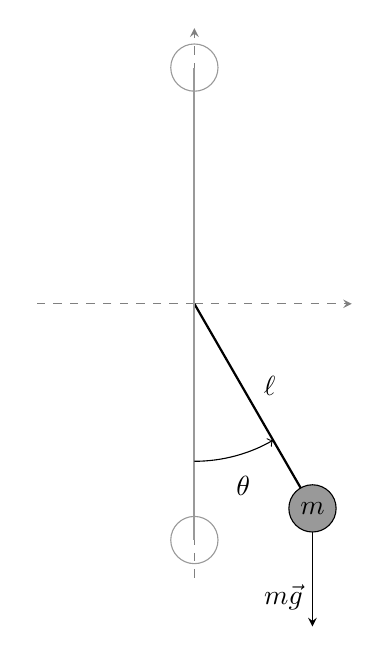
\begin{tikzpicture}
    % save length of g-vector and theta to macros
    \pgfmathsetmacro{\Gvec}{1.5}
    \pgfmathsetmacro{\myAngle}{30}
    
    \coordinate (centro) at (0,0);
    
    \draw[dashed,gray,-stealth] (centro) -- ++ (0,3.5) node (mary) [black,below]{$ $};
    \draw[dashed,gray,-stealth] (centro) -- ++ (2,0) node (mary) [black,below]{$ $};
    \draw[dashed,gray,-] (centro) -- ++ (-2,0) node (mary) [black,below]{$ $};
    \draw[dashed,gray,-] (centro) -- ++ (0,-3.5) node (mary) [black,below]{$ $};
    
    \draw[thick] (centro) -- node[above right] {$\ell$} ++(270+\myAngle:3) coordinate (bob) ;
    \draw[thick,draw=black!40] (centro) -- ++(270:3) coordinate (bob_0);
    \draw[thick,draw=black!40] (centro) -- ++(90:3) coordinate (bob_1);
    
    \pic [draw, ->, "$\theta$", angle eccentricity=1.2, angle radius = 2cm] {angle = mary--centro--bob};
    
    \draw [-stealth] (bob) -- ++(0,-\Gvec)
    coordinate (g)
    node[near end,left] {$m\vec{g}$};
    
    \filldraw [fill=black!40,draw=black] (bob) circle[radius=0.3] node {$m$} ;
    \filldraw [fill=none,draw=black!40] (bob_0) circle[radius=0.3];
    \filldraw [fill=none,draw=black!40] (bob_1) circle[radius=0.3];
    
\end{tikzpicture}

\end{document}